










\clearpage

\section{Further experimental details}
\label{app:further-experiments}
In this section we provide experimental details for each experiment, and report the results both visually and in terms of EMD and MMD.  We also showed how these metric change over 10 iterations of reference refinement. 

\subsection{Metric choice}
\label{app:metrics}
We choose to use two metrics that are commonly used in the literature to compare distributions, the Earth Mover Distance (EMD, \citet{rubner1998metric}, also known as Wasserstein-1) and the Maximum Mean Discrepancy (MMD, \citet{gretton2012kernel}). The EMD between two distributions $P$ and $Q$ can be defined by the maximization problem 
\begin{equation}
    \mathrm{EMD}(P,Q) = \sup_{||f||_L\le 1} \E_{x\sim P}f(x)-\E_{y\sim Q}f(y)
\end{equation} 
where $||f||_L\le 1$ constraints the function $f$ to be 1-Lipschitz continuous, i.e. $||\nabla f||\le 1$. The EMD intuitively measures the distance between two probability distributions by computing the minimum cost required to transform one distribution into the other. This metric allows us to quantify the similarity between the inferred and actual trajectories. This is a valid metric for our experiments, since if the inferred and actual trajectories are from the same distribution we expect it to converge to 0 (as the amount of trajectories goes to infinity). See \citet{fournier2015rate} for more details on this property. The metric can be calculated using the Sinkhorn algorithm. We use the implementation in the TrajectoryNet package. EMD is a widely used metric in the literature and remains useful in our setting because we work in low-dimensional spaces: our simulations are in 2D, and for the real data experiment, we reduce the data to the first five principal components. However, in higher-dimensional settings, EMD becomes less reliable due to the curse of dimensionality. Therefore, if a practitioner intends to apply our method to high-dimensional data, we recommend using MMD instead, as it is better suited for such cases.

The MMD between two distributions is defined in a very similar way. Instead of constraining the optimization problem to 1-Lipschitz continuous functions, we ask $f$ to be in a reproducing kernel Hilbert space $\mathcal{H}$ induced by a kernel function of choice.
\begin{equation}
    \mathrm{MMD}(P,Q) = \sup_{f\in\mathcal{H}} \E_{x\sim P}f(x)-\E_{y\sim Q}f(y)
\end{equation}

In our implementation, we pick the underlying kernel to be the Radial Basis Function (RBF) kernel with a length scale of 1 across all experiments. 

\subsection{Experiments tiebreaking details}
\label{app:tiebreaking}
In the tables across the paper, we highlight in green the method with lowest mean error over the restricted trajectories; we also highlight any other (restricted) method whose one-standard-deviation confidence interval overlaps the mean of the best (restricted) method. Separately, we use light blue to indicate any all-trajectory method whose one-standard-deviation confidence interval either overlaps with or falls below the mean of the best (restricted) method. 

\subsection{Lotka-Volterra}
\label{app:lv-app}
\subsubsection{Experiment setup}
For this experiment, we are interested in learning the dynamics of a stochastic Lotka-Volterra predator-prey model. The dynamics of the prey and predator populations are given by the following SDEs:
\begin{align}
\begin{split}
\label{eq:lv-family}
    dX &= \alpha X-\beta XY + 0.1dW_x\\
    dY &= \gamma XY-\delta Y + 0.1dW_y
\end{split}
\end{align}
where $[dW_x,dW_y]$ is a 2D Brownian motion.  

To obtain data, we fix the following parameters: $\alpha=1, \beta = 0.4, \gamma=0.1,\delta=0.4$. We start the dynamics at $X_0\sim U(5,5.1)$ and $Y_0\sim U(4,4.1)$, and simulate the SDEs for 10 instants of time. The length of each time interval is 1. We use Euler-Maruyama method to obtain the numeric solutions. We obtain 50 particles for each snapshot. We set $\Delta t = 0.01$ for every discretization step. We initialize the reference drift to 0, so that the initial reference SDE is a simple Brownian motion. 

\subsubsection{Reference family choice}
\label{app:LV_implementation}
 For this experiment, we have access to the data-generating process, as described in \cref{eq:lv-family}. Therefore, we select the reference family to be the set of SDEs that satisfy this system of equations, \cref{eq:lv-family}. We implement this reference family in practice as a PyTorch \texttt{nn.Module} with four scalar parameters, $\alpha, \beta, \gamma, \delta$. These parameters are to be learned during the optimization phase. Specifically, we use this module to evaluate $dX$ and $dY$, returning \texttt{torch.stack([dX, dY])} in the \texttt{nn.forward} method. The learning process involves optimizing the parameters using gradient descent, with a learning rate of 0.05 over 20 epochs, as determined by the grid search detailed in \cref{app:inverseproj}.


\subsubsection{Results} 
We provide a visual representation ot the trajectories in \cref{fig:LV-main} in the main text. In terms of EMD and MMD metrics, we show the results in \cref{tab:LV50_EMD_appendix} and \cref{tab:LV50_MMD}, respectively. We can see that our method is most of the times the best on the restricted set of trajectories (first four rows), and always at least as good as the other methods. When considering results over all possible trajectories (last two rows) our method is even better, especially for the last time step.

\begin{table*}[!ht]
    \centering
    \begin{tabular}{lcccc}
    \hline
        Method & EMD $t_2$ & EMD $t_4$ & EMD $t_6$ & EMD $t_8$ \\
    \hline
    \vanillaonetime & 0.59 $\pm$ 0.28 & 0.46 $\pm$ 0.073 & 0.40 $\pm$ 0.059 & \cellcolor{green!25}\textbf{0.70 $\pm$ 0.10} \\
         \dmsb & 0.49 $\pm$ 0.073 & 0.38 $\pm$ 0.12 & \cellcolor{green!25}\textbf{0.30 $\pm$ 0.11} & 0.84 $\pm$ 0.27\\
         \trajnet & 3.41 $\pm$ 0.050 & 1.27 $\pm$ 0.030 & 1.08 $\pm$ 0.040 & 3.99 $\pm$ 0.35 \\
         \oursonetime & \cellcolor{green!25}\textbf{0.22 $\pm$ 0.039} & \cellcolor{green!25}\textbf{0.16 $\pm$ 0.026} & \cellcolor{green!25}\textbf{0.31 $\pm$ 0.070} & \cellcolor{green!25}\textbf{0.74 $\pm$ 0.18} \\
    \hline
    \vanillaalltime & 0.59 $\pm$ 0.29 & 0.46 $\pm$ 0.074 & 0.38 $\pm$ 0.067 & \cellcolor{blue!10}\textbf{0.57 $\pm$ 0.072} \\
    \oursalltime & \cellcolor{blue!10}\textbf{0.21 $\pm$ 0.039} & \cellcolor{blue!10}\textbf{0.15 $\pm$ 0.021} & \cellcolor{blue!10}\textbf{0.30 $\pm$ 0.071} & \cellcolor{blue!10}\textbf{0.48 $\pm$ 0.055} \\
    \hline
    \end{tabular}
    \caption{Earth mover's distance (mean $\pm$ standard deviation) in four validation time points in Lotka-Volterra dataset with 50 particles each snapshot. Results were averaged over 10 seeds.}
    \label{tab:LV50_EMD_appendix}
\end{table*}


\begin{table*}[!ht]
    \centering
    \begin{tabular}{lcccc}
    \hline
        Method & MMD $t_2$ & MMD $t_4$ & MMD $t_6$ & MMD $t_8$ \\
    \hline
        \vanillaonetime & 2.73 \fpm 2.08 & 1.63 \fpm 0.54 & 0.68 \fpm 0.38 & \cellcolor{green!25}\textbf{0.78 \fpm 0.26} \\
         \dmsb & 2.03 $\pm$ 0.51 & 1.06 $\pm$ 0.69 & \cellcolor{green!25}\textbf{0.48 $\pm$ 0.36} & 1.26 $\pm$ 0.72\\
         \trajnet & 7.27 $\pm$ 0.11 & 6.33 $\pm$ 0.33 & 5.34 $\pm$ 0.20 & 6.35 $\pm$ 0.33 \\
         \oursonetime & \cellcolor{green!25}\textbf{0.40 \fpm 0.16} & \cellcolor{green!25}\textbf{0.068 \fpm 0.069} & \cellcolor{green!25}\textbf{0.34 \fpm 0.25} & \cellcolor{green!25}\textbf{0.80 \fpm 0.44} \\
    \hline
        \vanillaalltime & 2.75 $\pm$ 2.11 & 1.63 $\pm$ 0.55 & \cellcolor{blue!10}\textbf{0.67 $\pm$ 0.39} & \cellcolor{blue!10}\textbf{0.62 $\pm$ 0.23} \\    
        \oursalltime & \cellcolor{blue!10}\textbf{0.38 $\pm$ 0.16} & \cellcolor{blue!10}\textbf{0.05 $\pm$ 0.03} & \cellcolor{blue!10}\textbf{0.33 $\pm$ 0.25} & \cellcolor{blue!10}\textbf{0.29 $\pm$ 0.11} \\
    \hline
    \end{tabular}
    \caption{Maximum mean discrepancy (mean $\pm$ standard deviation) in four validation time points in Lotka-Volterra dataset with 50 particles. Results averaged over 10 seeds.}
    \label{tab:LV50_MMD}
\end{table*}




\clearpage


\subsection{Repressilator}
\label{app:repr-app}

\subsubsection{Experiment setup} 
The repressilator is a synthetic genetic regulatory network that functions as a biological oscillator, or a genetic clock. It was designed to exhibit regular, sustained oscillations in the concentration of its components. The repressilator system consists of a network of three genes that inhibit each other in a cyclic manner: each gene produces a protein that represses the next gene in the loop, with the last one repressing the first, forming a feedback loop.

We can model the dynamics of the repressilator using the following SDEs:
\begin{align}
\label{eq:repr-family}
    dX_1&=\frac{\beta}{1+(X_3/k)^n}-\gamma X_1+0.1dW_1 \nonumber \\
    dX_2&=\frac{\beta}{1+(X_1/k)^n}-\gamma X_2+0.1dW_2\\
    dX_3&=\frac{\beta}{1+(X_2/k)^n}-\gamma X_3+0.1dW_3 \nonumber
\end{align}
where $[dW_1,dW_2,dW_3]$ is a 3D Brownian motion, and the repressing behavior is quite clear from the drift equations. 

To obtain data, we fix the following parameters: $\beta = 10, n=3, k = 1, \gamma = 1$. We start the dynamics with initial distribution $X_1, X_2\sim U(1,1.1)$ and $X_3\sim U(2,2.1)$. We simulate the SDEs for 10 instants of time. At each time step, we take 50 samples. We use Euler-Maruyama method to obtain the numeric solutions. Also for this experiment, we set $\Delta t = 0.01$ for every discretization step. We initialize the reference drift to 0, so that the initial reference SDE is a simple Brownian motion.

\subsubsection{Reference family choice}
\label{app:repr_implementation}
For this experiment, we have access to the data-generating process, as described in \cref{eq:repr-family}. Therefore, we select the reference family to be the set of SDEs that satisfy this system of equations, \cref{eq:repr-family}. We implement this reference family in practice as a PyTorch \texttt{nn.Module} with four scalar parameters \(\beta, n, k, \gamma\) to be optimized by gradient descent. Specifically, we use this module to evaluate \(dX_1, dX_2\), and \(dX_3\), returning \texttt{torch.stack([$dX_1, dX_2, dX_3$])} in the \texttt{nn.forward} method. The learning process involves optimizing the parameters using gradient descent, with a learning rate of 0.05 over 20 epochs, as determined by the grid search detailed in \cref{app:inverseproj}.

\subsubsection{Results.} We provide a visual representation ot the trajectories in \cref{fig:repr-main} in the main text. In terms of EMD and MMD metrics, we show the results in \cref{tab:repres50_EMD_appendix} and \cref{tab:repres50_MMD}, respectively. We can see that our method is in general better than all the other methods on the restricted set of trajectories (first four rows), besides the last time point where \vanilla{} is the best. When considering results over all possible trajectories (last two rows), our method becomes even better at some time steps (especially $t_6$. \vanilla{} shows similar performance.


\begin{table*}[!ht]
    \centering
    \begin{tabular}{lccccc}
    \hline
        Method & EMD $t_2$ & EMD $t_4$ & EMD $t_6$ & EMD $t_8$ & EMD $t_{10}$ \\
    \hline
        \vanillaonetime& 1.87 $\pm$ 0.047 & 1.22 $\pm$ 0.12 & 1.33 $\pm$ 0.17 & \cellcolor{green!25}\textbf{1.20 $\pm$ 0.18} & \cellcolor{green!25}\textbf{1.16 $\pm$ 0.14} \\
         \dmsb & 1.46 $\pm$ 0.08 & 1.08 $\pm$ 0.37 & 3.00 $\pm$ 0.54 & 2.18 $\pm$ 0.41 & 2.54 $\pm$ 1.21\\
         \trajnet & 3.62 $\pm$ 0.05 & 2.86 $\pm$ 0.08 & 1.67 $\pm$ 0.07 & 3.45 $\pm$ 0.09 & 2.33 $\pm$ 0.08 \\
         \oursonetime & \cellcolor{green!25}\textbf{0.51 $\pm$ 0.11} & \cellcolor{green!25}\textbf{0.76 $\pm$ 0.10} & \cellcolor{green!25}\textbf{0.49 $\pm$ 0.10} & \cellcolor{green!25}\textbf{1.25 $\pm$ 0.27} & 2.18 $\pm$ 0.58 \\
    \hline
    \vanillaalltime & 1.87 $\pm$ 0.05 & 1.23 $\pm$ 0.10 & 1.27 $\pm$ 0.15 & \cellcolor{blue!10}\textbf{1.19 $\pm$ 0.13} & \cellcolor{blue!10}\textbf{1.16 $\pm$ 0.14} \\
    \oursalltime & \cellcolor{blue!10}\textbf{0.50 $\pm$ 0.11} & 0.87 $\pm$ 0.10 & \cellcolor{blue!10}\textbf{0.51 $\pm$ 0.09} & \cellcolor{blue!10}\textbf{0.61 $\pm$ 0.10} & 1.49 $\pm$ 0.20 \\
    \hline
    \end{tabular}
    \caption{Earth mover's distance (mean $\pm$ standard deviation) in five validation time points in repres50 dataset, our method performs better than the baseline SB.}
    \label{tab:repres50_EMD_appendix}
\end{table*}



\begin{table*}[!ht]
    \centering
    \begin{tabular}{lccccc}
    \hline
        Method & MMD $t_2$ & MMD $t_4$ & MMD $t_6$ & MMD $t_8$ & MMD $t_{10}$ \\
    \hline
        \vanillaonetime & 9.33 \fpm 0.059 & 5.52 \fpm 0.68 & 4.19 \fpm 0.68 & \cellcolor{green!25}\textbf{1.87 \fpm 0.62} & \cellcolor{green!25}\textbf{2.04 \fpm 0.50} \\
         \dmsb & 8.07 $\pm$ 0.29 & 4.37 $\pm$ 1.54 & 5.75 $\pm$ 0.37 & 3.65 $\pm$ 0.97 & 2.30 $\pm$ 0.83\\
         \trajnet & 6.86 $\pm$ 0.06 & 6.23 $\pm$ 0.13 & 4.56 $\pm$ 0.17 & 5.40 $\pm$ 0.33 & 4.61 $\pm$ 0.26 \\
         \oursonetime & \cellcolor{green!25}\textbf{1.97 \fpm 0.80} & \cellcolor{green!25}\textbf{2.70 \fpm 0.66} & \cellcolor{green!25}\textbf{0.60 \fpm 0.32} & \cellcolor{green!25}\textbf{1.40 \fpm 0.51} & \cellcolor{green!25}\textbf{2.20 \fpm 0.96}\\
    \hline
    \vanillaalltime & 9.33 $\pm$ 0.06 & 5.31 $\pm$ 0.72 & 3.87 $\pm$ 0.75 & \cellcolor{blue!10}\textbf{1.74 $\pm$ 0.69} & \cellcolor{blue!10}\textbf{1.70 $\pm$ 0.52} \\
    \oursalltime & \cellcolor{blue!10}\textbf{1.96 $\pm$ 0.80} & 3.34 $\pm$ 0.50 & \cellcolor{blue!10}\textbf{0.64 $\pm$ 0.24} & \cellcolor{blue!10}\textbf{0.51 $\pm$ 0.18} & \cellcolor{blue!10}\textbf{0.95 $\pm$ 0.23} \\
    \hline
    \end{tabular}
    \caption{Maximum mean discrepancy (mean $\pm$ standard deviation) in five validation time points in repres50 dataset.}
    \label{tab:repres50_MMD}
\end{table*}

\clearpage

\subsection{Gulf of Mexico vortex data}
\label{app:GoM-app}
\subsubsection{Experiment setup}
\label{app:GoM-app-exp-details}

In this experiment, we test our method on real ocean-current data from the Gulf of Mexico. We use high-resolution (1 km) bathymetry data from a HYbrid Coordinate Ocean Model (HYCOM) reanalysis\footnote{Dataset available at \href{https://www.hycom.org/data/gomb0pt01/gom-reanalysis}{this link}.} \citep{panagiotis2014gulf}. This dataset was released by the US Department of Defense, and is thus of public domain. The dataset provides hourly ocean current velocity fields for the region extending from 98$^{\circ}$E to 77$^{\circ}$E in longitude and from 18$^{\circ}$N to 32$^{\circ}$N in latitude, covering every day since January 1\textsuperscript{st}, 2001. We focus on a specific time point, June 1st 2024 at 5pm at surface level, and a particular spatial region where a vortex is observed. By doing so, we obtain a unique velocity field with a known general behavior. Using this field, we generate particles that evolve according to the ocean currents while satisfying our modeling assumptions. Specifically, we select an initial location near the vortex and uniformly sample 1,000 initial positions within a small radius ($0.05$) around this point, representing the starting positions of 1,000 particles. We then evolve these particles over nine time steps using the ocean current velocity field. The time step size is $0.9$. Since the velocity field is defined on a fine grid, we approximate the velocity at each particle's position by using the velocity at the nearest grid point when the particle does not align exactly with a grid point. This approach simulates the particles' trajectories within the system. To create data that align with our modeling assumptions, we randomly assign each particle to one of the nine time steps, ensuring that (1) each particle is observed at only one time point, and (2) each time step has approximately the same number of particle observations. Specifically, we observe about 111 particles at each time step (since $1,000 \div 9 \approx 111$). This results in a dataset with sparse observations, where individual particle trajectories are not fully observed. We perform this data generation task twice, starting at two different locations around the vortex. See \cref{fig:gomdata} for a visual representation. We refer to the data in the left plot of \cref{fig:gomdata} as \textit{Gulf of Mexico - big vortex}. And to the data in the right plot as \textit{Gulf of Mexico - small vortex}. The goal of this experiment is to assess whether our method and the baseline methods can reconstruct the vortex from these two sparse particle datasets without access to complete individual trajectories.


\begin{figure}
    \centering
    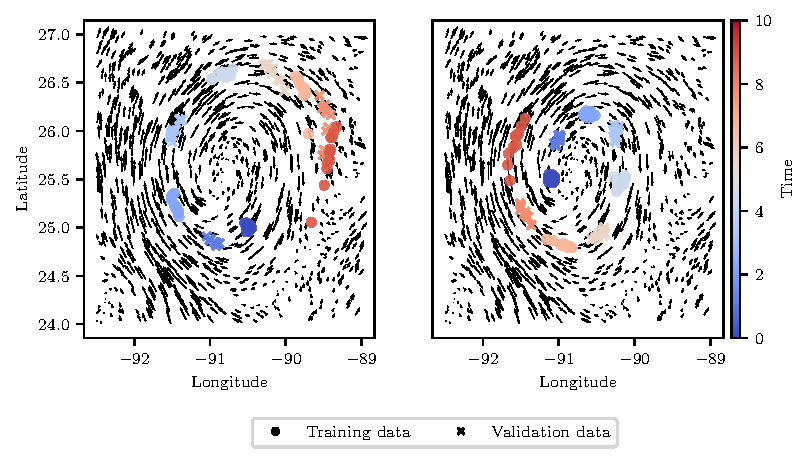
\includegraphics[width=0.8\linewidth]{Ch3-SBIRR/Figs/GoM_data.pdf}
    \caption{Our two datasets and the underlying ocean current dynamics from which we generated the data (black arrows). Left: \textit{Gulf of Mexico - big vortex} experiment. Right: \textit{Gulf of Mexico - small vortex} experiment. }
    \label{fig:gomdata}
\end{figure}

\subsubsection{Reference family choice} 
\label{app:GoM-app-reference}

For this real data experiment, we do not have access to the data-generating process. However, we can leverage domain knowledge about the underlying ocean current vortex dynamics. Specifically, we model the dynamics of the vortex using the following SDEs:

\begin{align}
\label{eq:vortex-family}
    dX_1 & =\texttt{scale} \cdot \bigg((X_2 - X_2^{\text{center}}) \cdot \exp{(-\texttt{logyscale})}\bigg) \nonumber +0.1dW_1 \\
    dX_2 &= -\texttt{scale} \bigg(X_1 - X_1^{\text{center}}\bigg)\nonumber+0.1dW_2
\end{align}
This is a standard constant curl representation for a vortex of scale $\texttt{scale}$, centered at \(dX_1, dX_2\), with a potential elliptical deformation determined by $\texttt{logyscale}$. We implement this reference family in practice as a PyTorch \texttt{nn.Module} with four scalar parameters, $X_1^{\text{center}}, X_2^{\text{center}}, \texttt{logyscale}$ and $\texttt{scale}$ to be learned by gradient descent. This module is then used to evaluate \(dX_1, dX_2\), returning \texttt{torch.stack([$dX_1, dX_2$])} in the \texttt{nn.forward} method. The learning process involves optimizing the parameters using gradient descent, with a learning rate of 0.05 over 20 epochs, as determined by the grid search described in \cref{app:inverseproj}.

\subsubsection{Results.}
\label{app:GoM-app-results}

We provide a visual representation ot the trajectories for the small vortex in \cref{fig:GoMsmall-main} in the main text and for the big vortex in \cref{fig:GoM-appendix}. In terms of EMD and MMD metrics, we show the results for the small vortex in \cref{tab:GoMsmall_EMD_appendix} and \cref{tab:GoMvortexsmall_MMD}, respectively. And for the big vortex in \cref{tab:GoMlarge_EMD_appendix} and \cref{tab:GoMvortex_MMD}. 

For the small vortex, we can see that our method has similar performance to \dmsbname{} on the restricted set of trajectories. And these two methods are both better than the other two alternatives. When considering results over all possible trajectories (last two rows), our method performs even better. If we look at \cref{fig:GoMsmall-main}, we can see that \vanilla{} fails to capture the curvature. \dmsbname{} and TrajectoryNet generate smooth trajectories that are notably far from the data the final validation time point. Our trajectories track the curvature of the validation data closely.

Similar results are observed for the big vortex experiment. Our method has similar performance to \dmsbname{} on the restricted set of trajectories. In particular, according to EMD \dmsbname{} is better for the first time step, similar for the second, and worse for the last two. By comparing the trajectories visually in \cref{fig:GoM-appendix}, we also see that \vanilla{} fails to capture the curvature. \dmsbname{} generates smooth trajectories that fail to capture the third validation time point (and have a slightly unnatural shape in the top right corner of the figure). TrajectoryNet generate smooth trajectories that fail to capture the first validation time point. Our model generates trajectories that most closely resembles the shape that we observe in the ocean current in \cref{fig:gomdata}.


\begin{table*}[!ht]
    \centering
    \begin{tabular}{lcccc}
    \hline
        Method & EMD $t_2$ & EMD $t_4$ & EMD $t_6$ & EMD $t_8$ \\
    \hline
    \vanillaonetime & 0.27 $\pm$ 0.060 & 0.30 $\pm$ 0.056 & 0.43 $\pm$ 0.053 & 0.42 $\pm$ 0.048 \\
   
     
        
         \dmsb & \cellcolor{green!25}\textbf{0.086 $\pm$ 0.011} & \cellcolor{green!25}\textbf{0.092 $\pm$ 0.020} & \cellcolor{green!25}\textbf{0.088 $\pm$ 0.009} & 0.21 $\pm$ 0.027\\
         \trajnet & 0.78  $\pm$ 0.014 & 0.77$\pm$0.048 & 1.19$\pm$0.15 & 0.76$\pm$0.17 \\
         \oursonetime & \cellcolor{green!25}\textbf{0.075 $\pm$ 0.023} & \cellcolor{green!25}\textbf{0.080 $\pm$ 0.017} & 0.13 $\pm$ 0.037 & \cellcolor{green!25}\textbf{0.11 $\pm$ 0.032} \\
    \hline
     \vanillaalltime & 0.27 $\pm$ 0.058 & 0.30 $\pm$ 0.056 & 0.42 $\pm$ 0.056 & 0.41 $\pm$ 0.048 \\
   \oursalltime & \cellcolor{blue!10}\textbf{0.073 $\pm$ 0.020} & \cellcolor{blue!10}\textbf{0.072 $\pm$ 0.012} & 0.12 $\pm$ 0.029 & \cellcolor{blue!10}\textbf{0.094 $\pm$ 0.023} \\
    \hline
    \end{tabular}
    \caption{Earth mover's distance (mean $\pm$ standard deviation) in four validation time points in Gulf of Mexico - small vortex dataset. Results were averaged over 10 seeds.}
    \label{tab:GoMsmall_EMD_appendix}
\end{table*}

\begin{figure*}[!ht]
    \centering
    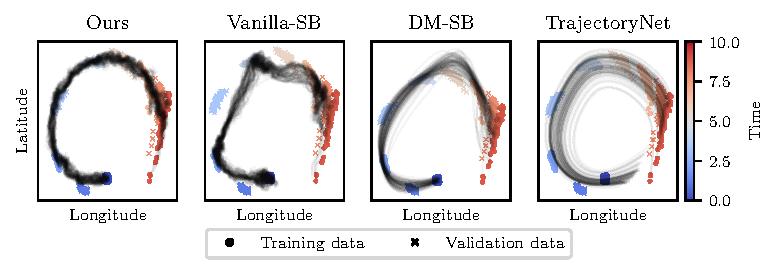
\includegraphics[width =0.9\textwidth]{Ch3-SBIRR/Figs/GoM_trajectories.pdf}
    \caption{ Comparison on the Gulf of Mexico - big vortex data with 5 training times, 4 validation times, and approximately 111 observations per time. Each plot shows approximately 111 simulated trajectories, originating from particles at one time end point (three left plots: first time; right plot: final time).} 
    \label{fig:GoM-appendix}
\end{figure*}


\begin{table*}[!ht]
    \centering
    \begin{tabular}{lcccc}
    \hline
        Method & EMD $t_2$ & EMD $t_4$ & EMD $t_6$ & EMD $t_8$ \\
    \hline
     \vanillaonetime & 0.35 $\pm$ 0.043 & 0.55 $\pm$ 0.067 & 0.42 $\pm$ 0.047 & 0.21 $\pm$ 0.038 \\
         
         \dmsb & \cellcolor{green!25}\textbf{0.074 $\pm$ 0.029} & \cellcolor{green!25}\textbf{0.12 $\pm$ 0.027} & 0.19 $\pm$  0.040  & 0.17 $\pm$ 0.048\\
         \trajnet & 1.94  $\pm$ 0.015 & 1.37$\pm$0.043 & 1.27$\pm$0.10 & 1.68$\pm$0.11 \\
         \oursonetime & 0.19 $\pm$ 0.044 & \cellcolor{green!25}\textbf{0.13 $\pm$ 0.038} & \cellcolor{green!25}\textbf{0.092 $\pm$ 0.021} & \cellcolor{green!25}\textbf{0.13 $\pm$ 0.020} \\
    \hline
    \vanillaalltime & 0.35 $\pm$ 0.043 & 0.55 $\pm$ 0.071 & 0.41 $\pm$ 0.050 & 0.20 $\pm$ 0.035 \\
     \oursalltime & 0.20 $\pm$ 0.038 & \cellcolor{blue!10}\textbf{0.13 $\pm$ 0.040} & \cellcolor{blue!10}\textbf{0.086 $\pm$ 0.020} & \cellcolor{blue!10}\textbf{0.13 $\pm$ 0.017} \\
    \hline
    \end{tabular}
    \caption{Earth mover's distance (mean $\pm$ standard deviation) in four validation time points in Gulf of Mexico - big vortex dataset. Results were averaged over 10 seeds.}
    \label{tab:GoMlarge_EMD_appendix}
\end{table*}

\begin{table*}[!ht]
    \centering
    \begin{tabular}{lcccc}
    \hline
        Method & MMD $t_2$ & MMD t=2 & MMD $t_4$ & MMD t=4 \\
    \hline
    \vanillaonetime & 0.73 \fpm 0.32&  0.86\fpm 0.33& 1.67\fpm 0.37 & 1.48\fpm 0.32 \\
         \dmsb & \cellcolor{green!25}\textbf{0.07 $\pm$ 0.02} & 0.08 $\pm$ 0.04 & \cellcolor{green!25}\textbf{0.06 $\pm$ 0.02} & 0.34 $\pm$ 0.11 \\
         \trajnet & 4.38 $\pm$ 0.25 & 4.38 $\pm$ 0.40 & 7.36 $\pm$ 0.76 & 4.16 $\pm$ 1.28 \\
         \oursonetime & \cellcolor{green!25}\textbf{0.042 \fpm 0.035} & \cellcolor{green!25}\textbf{0.043 \fpm 0.031} & 0.16 \fpm 0.10 & \cellcolor{green!25}\textbf{0.064 \fpm 0.031} \\
         
    \hline
    
    \vanillaalltime & 0.72 $\pm$ 0.30 & 0.87 $\pm$ 0.34 & 1.67 $\pm$ 0.39 & 1.44 $\pm$ 0.32 \\

    \oursalltime & \cellcolor{blue!10}\textbf{0.04 $\pm$ 0.03} & \cellcolor{blue!10}\textbf{0.03 $\pm$ 0.02} & 0.14 $\pm$ 0.07 & \cellcolor{blue!10}\textbf{0.05 $\pm$ 0.04} \\
    \hline
    \end{tabular}
    \caption{Maximum mean discrepancy (mean $\pm$ standard deviation) in four validation time points in Gulf of Mexico - small vortex dataset. Results were averaged over 10 seeds.}
    \label{tab:GoMvortexsmall_MMD}
\end{table*}



\begin{table*}[!ht]
    \centering
    \begin{tabular}{lcccc}
    \hline
        Method & MMD $t_2$ & MMD t=2 & MMD $t_4$ & MMD t=4 \\
    \hline
         \vanillaonetime & 1.11 \fpm 0.26& 2.52\fpm  0.53& 1.25\fpm  0.32& 0.27\fpm  0.14 \\
         \dmsb & \cellcolor{green!25}\textbf{0.05 $\pm$ 0.05} & \cellcolor{green!25}\textbf{0.10 $\pm$ 0.07} & \cellcolor{green!25}\textbf{0.30 $\pm$ 0.15} & \cellcolor{green!25}\textbf{0.19 $\pm$ 0.13} \\
         \trajnet & 9.40 $\pm$ 0.04 & 8.19 $\pm$ 0.20 & 7.72 $\pm$ 0.53 & 8.92 $\pm$ 0.17 \\
         \oursonetime & 0.35 \fpm 0.17 & \cellcolor{green!25}\textbf{0.15\fpm  0.10} & \cellcolor{green!25}\textbf{0.42\fpm  0.031} & 0.49\fpm  0.028\\
         \hline
         \vanillaalltime & 1.14 $\pm$ 0.26 & 2.53 $\pm$ 0.55 & 1.50 $\pm$ 0.34 & \cellcolor{blue!10}\textbf{0.27 $\pm$ 0.13} \\
         \oursalltime & 0.37 $\pm$ 0.15 & \cellcolor{blue!10}\textbf{0.13 $\pm$ 0.09} & \cellcolor{blue!10}\textbf{0.04 $\pm$ 0.03} & \cellcolor{blue!10}\textbf{0.06 $\pm$ 0.03} \\
    \hline
    \end{tabular}
    \caption{Maximum mean discrepancy (mean $\pm$ standard deviation) in four validation time points in Gulf of Mexico - big vortex dataset. Results were averaged over 10 seeds.}
    \label{tab:GoMvortex_MMD}
\end{table*}




\clearpage

\subsection{Single cell datasets}
\label{app:eb-app}

\subsubsection{Experiment setup} 
\label{app:singlecellsetup}
We consider two different single cell data for this experiment: the one from \citet{moon2019visualizing} on embryoid body cells (EB) and the one from \citet{chu2016single} on human embryonic stem cells (hESC). Both datasets are shared under CC-by-4.0 license. Both datasets offer insights into the dynamic process of stem cell differentiation by capturing gene expression levels at different stages.
\citet{tong2020trajectorynet} applied a pre-processing pipeline, including dimensionality reduction via Principal Component Analysis, to the EB data. We use the same pre-processing for the EB data; we apply the same pipeline to the hESC data as well. The EB dataset consists of five snapshots that are largely overalapping so we subsampled it to have 300 cells at each snapshot. The hESC dataset initially consists of six snapshots. Note that we want validation data at every other snapshot, and we also want the first and last snapshot to serve as training points. Therefore, we want the total number of snapshots to be an odd number. To meet this desideratum, we choose to ignore the last snapshot of the hESC data. The EB data already meets this desideratum. To apply our method to this dataset, we set $\Delta t = 0.01$ for every discretization step involving SDEs. We initialize the reference drift to 0, so that the initial reference SDE is a simple Brownian motion.

\subsubsection{Reference family choice} 
\label{app:eb_implementation}
For this experiment, we do not have access to the data generating process, so we cannot proceed as done for the synthetic experiments. Nonetheless, scientists have domain knowledge about the underlying dynamics of cell differentiation process. In particular, following \citet{wang2011quantifying, weinreb2018fundamental, lavenant2024toward}, we use a gradient field family. This family is motivated by Waddington's famous analogy between cellular differentiation and a marble rolling down a potential surface \citep{waddington2014strategy}. In practice, we parameterize the gradient field using a multilayer perceptron, an architecture used for gradient field in literature \citep[e.g.,][]{greydanus2019hamiltonian,lin2023computing}. We tested several potential models with one hidden layer of size 128, two hidden layers of size 128 and 64, three hidden layers of sizes 128, 64, and 64, and three hidden layers of sizes 128, 128, and 64 connected by ReLU activation functions, trained with learning rate 0.01 with 20 epochs. We choose based on the criteria described in \cref{app:inverseproj}. The final training hyperparameters is set to 0.01 and we trained for 50 epochs, chosen by the grid search criteria described in \cref{app:inverseproj} after choosing the architecture.


\subsubsection{Results.} In terms of visual reconstruction, \cref{fig:eb-app} shows that all the methods perform well in reconstructing trajectories in the EB experiments. This success can be attributed to the limited number of time steps, which results in restricted global information. Nonetheless, the trajectories for our method, \vanilla{}, and TrajectoryNet look more reasonable at interpolating the data. If we consider instead \cref{fig:hesc-app}, we can see how for this dataset it is very clear that both our method, \vanilla{}, and TrajectoryNet outperform \dmsbname. This approach, indeed, unfortunately seems unable to capture trajectories going through the observations in a meaningful way, whereas the other methods come up with trajectories that are visually reasonable given the observed data. This contradicts what we see in \cref{tab:EB_EMD_appendix} and \cref{tab:EB_MMD}. Indeed, when comparing the quality of only those trajectories generated from a single end point in time, \dmsbname{} outperforms the alternatives, including our method, for both EMD and MMD. However, when allowed to generate trajectories from all particles, \vanilla{} and our method outperform the single-time trajectory options (as expected) and perform comparably to each other.



\begin{figure}[!ht]
    \centering
    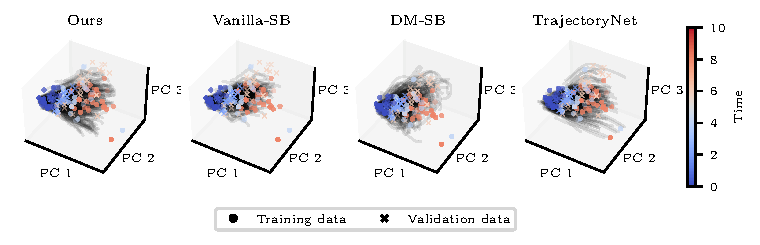
\includegraphics[width=\textwidth]{Ch3-SBIRR/Figs/eb_trajectories.pdf}
    \caption{EB dataset}
    \label{fig:eb-app}
\end{figure}

\begin{figure}[!ht]
    \centering
    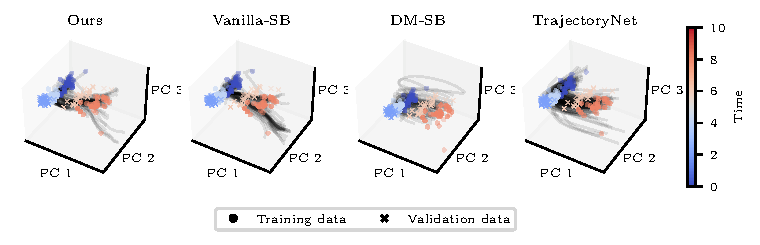
\includegraphics[width=\textwidth]{Ch3-SBIRR/Figs/hESC_trajectories.pdf}
    \caption{hESC dataset}
    \label{fig:hesc-app}
\end{figure}



\begin{table*}[!ht]
    \centering
    \begin{tabular}{lcccc}
    \hline
       & \multicolumn{2}{c}{EB} & \multicolumn{2}{c}{hESC} \\
        Method & EMD $t_2$ & EMD $t_4$ & EMD $t_2$ & EMD $t_4$ \\
    \hline
        \vanillaonetime & 1.49 $\pm$ 0.063 & 1.55 $\pm$ 0.034 & 1.47 $\pm$ 0.088 & 1.97 $\pm$ 0.169\\
         \dmsb & \cellcolor{green!25}\textbf{1.13 $\pm$ 0.082} & \cellcolor{green!25}\textbf{1.45 $\pm$ 0.16} & \cellcolor{green!25}\textbf{1.10 $\pm$ 0.066} & 1.51 $\pm$ 0.11\\
         \trajnet & 2.03 $\pm$ 0.04 & 1.93 $\pm$ 0.08 & 1.30 $\pm$ 0.04 & 1.93 $\pm$ 0.05 \\
         \oursonetime & 1.27 $\pm$ 0.028 & 1.57 $\pm$ 0.048 & \cellcolor{green!25}\textbf{1.08 $\pm$ 0.12} & \cellcolor{green!25}\textbf{1.33 $\pm$ 0.084} \\
    \hline
        \vanillaalltime & \cellcolor{blue!10}\textbf{1.12 $\pm$ 0.031} & \cellcolor{blue!10}\textbf{1.12 $\pm$ 0.023} & \cellcolor{blue!10}\textbf{0.72 $\pm$ 0.017} & \cellcolor{blue!10}\textbf{1.27 $\pm$ 0.043} \\
        \oursalltime & \cellcolor{blue!10}\textbf{0.96 $\pm$ 0.019} & \cellcolor{blue!10}\textbf{1.19 $\pm$ 0.017} & \cellcolor{blue!10}\textbf{0.71 $\pm$ 0.031} & \cellcolor{blue!10}\textbf{1.25 $\pm$ 0.076} \\
    \hline
    \end{tabular}
    \caption{Earth mover's distance (mean $\pm$ standard deviation) in two validation time points in EB and hESC datasets.}
    \label{tab:EB_EMD_appendix}
\end{table*}





% EB Dataset

\begin{table*}[!ht]
    \centering
    \begin{tabular}{lcccc}
    \hline
       & \multicolumn{2}{c}{EB} & \multicolumn{2}{c}{hESC} \\
        Method & MMD $t_2$ & MMD $t_4$ & MMD $t_2$ & MMD $t_4$ \\
    \hline
        \vanillaonetime & 0.68 \fpm 0.035  & 0.65 \fpm  0.066 & 5.23 \fpm  0.24  & 5.19  \fpm  0.22 \\
         
         \dmsb & \cellcolor{green!25}\textbf{0.24 $\pm$ 0.035} & \cellcolor{green!25}\textbf{0.19 $\pm$ 0.038} & \cellcolor{green!25}\textbf{3.22 $\pm$ 0.21} & \cellcolor{green!25}\textbf{3.23 $\pm$ 0.27} \\
         \trajnet & 0.62 $\pm$ 0.02 & 0.60 $\pm$ 0.10 & 4.03 $\pm$ 0.16 & 4.42 $\pm$ 0.17 \\
         \oursonetime & 0.45 \fpm 0.022 & 0.54 \fpm 0.081 & 3.71 \fpm 0.43 & \cellcolor{green!25}\textbf{3.49 \fpm 0.50} \\
    \hline
        \vanillaalltime & \cellcolor{blue!10}\textbf{0.19 $\pm$ 0.021} & \cellcolor{blue!10}\textbf{0.19 $\pm$ 0.017} & \cellcolor{blue!10}\textbf{1.85 $\pm$ 0.11} & \cellcolor{blue!10}\textbf{2.77 $\pm$ 0.17} \\
        \oursalltime & \cellcolor{blue!10}\textbf{0.14 $\pm$ 0.015} & \cellcolor{blue!10}\textbf{0.16 $\pm$ 0.011} & \cellcolor{blue!10}\textbf{2.02 $\pm$ 0.19} & \cellcolor{blue!10}\textbf{3.35 $\pm$ 0.30} \\
    \hline
    \end{tabular}
    \caption{Maximum mean discrepancy (mean $\pm$ standard deviation) in two validation time points in EB and hESC datasets.}
    \label{tab:EB_MMD}
\end{table*}

\clearpage

\subsection{Convergence Analysis of Test Metrics Across Iterations}
\label{app:multisteps-app}
In this section, we present the evolution of the test metrics --- MMD and EMD --- over ten iterative reference steps in our proposed method. Figures \ref{fig:emditer} and \ref{fig:mmditer} illustrate how these metrics change across different experimental settings. Specifically, \ref{fig:emditer} depicts the EMD at various validation time points, while \ref{fig:mmditer} displays the MMD trends over the same iterations. Our observations indicate that in most cases, the method exhibits initial improvements within the first few iterations, leading to a decrease in both EMD and MMD. Typically, ten iterations are sufficient for the refinement steps to reach stability, confirming the effectiveness of our iterative approach. However, in some validation steps --- such as the first two steps in the Repressilator experiment --- an increase in the test metric is observed after initial improvements, suggesting possible overfitting. This phenomenon highlights the importance of developing principled stopping criteria to prevent performance degradation beyond a certain number of iterations. These results provide insights into the iterative refinement behavior of our method and suggest potential directions for future work in adaptive stopping mechanisms.

\begin{figure}[!h]
    \centering
    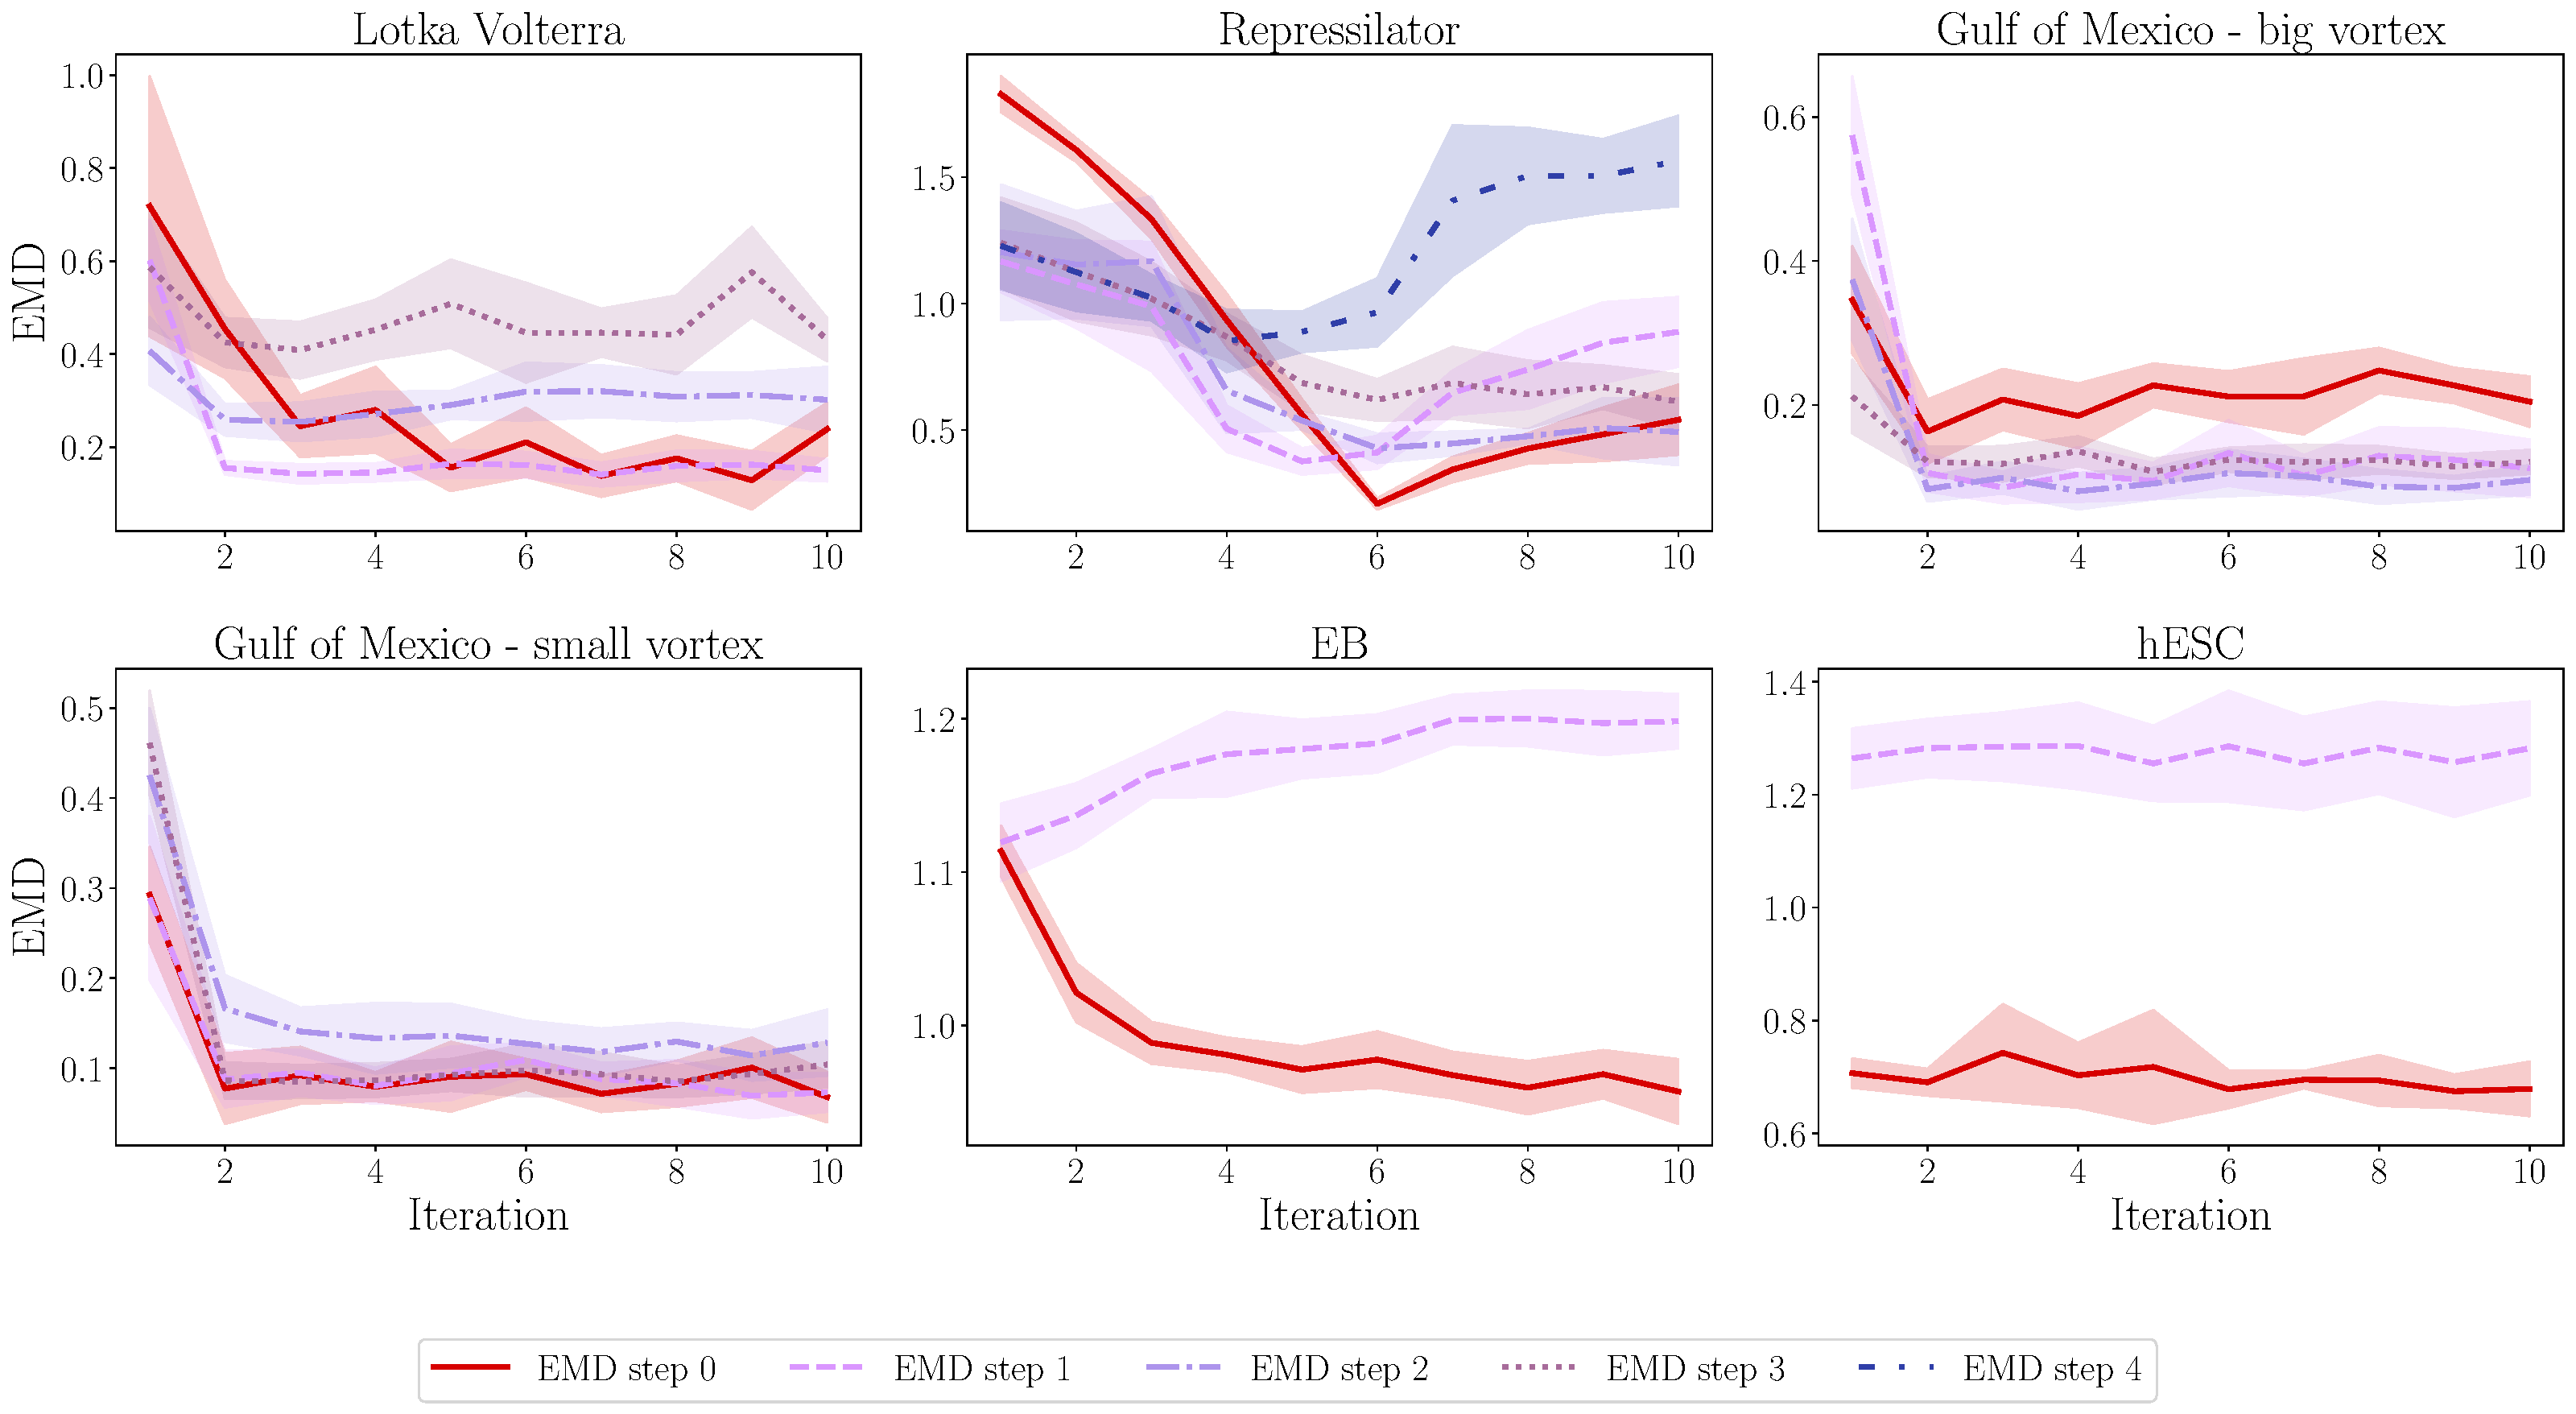
\includegraphics[width=\linewidth]{Ch3-SBIRR/Figs/EMD_eachiter_all.pdf}
    \caption{Evolution of the EMD metric across ten iterative refinement steps in our proposed method for different experimental settings. Each subplot corresponds to a specific experiment: Lotka-Volterra, Repressilator, Gulf of Mexico (big vortex), Gulf of Mexico (small vortex), EB, and hESC. The x-axis represents the iteration number, ranging from 1 to 10, while the y-axis indicates the EMD value at each validation time point. The different curves within each subplot correspond to the EMD measured at multiple validation steps.}
    \label{fig:emditer}
\end{figure}

\begin{figure}[!h]
    \centering
    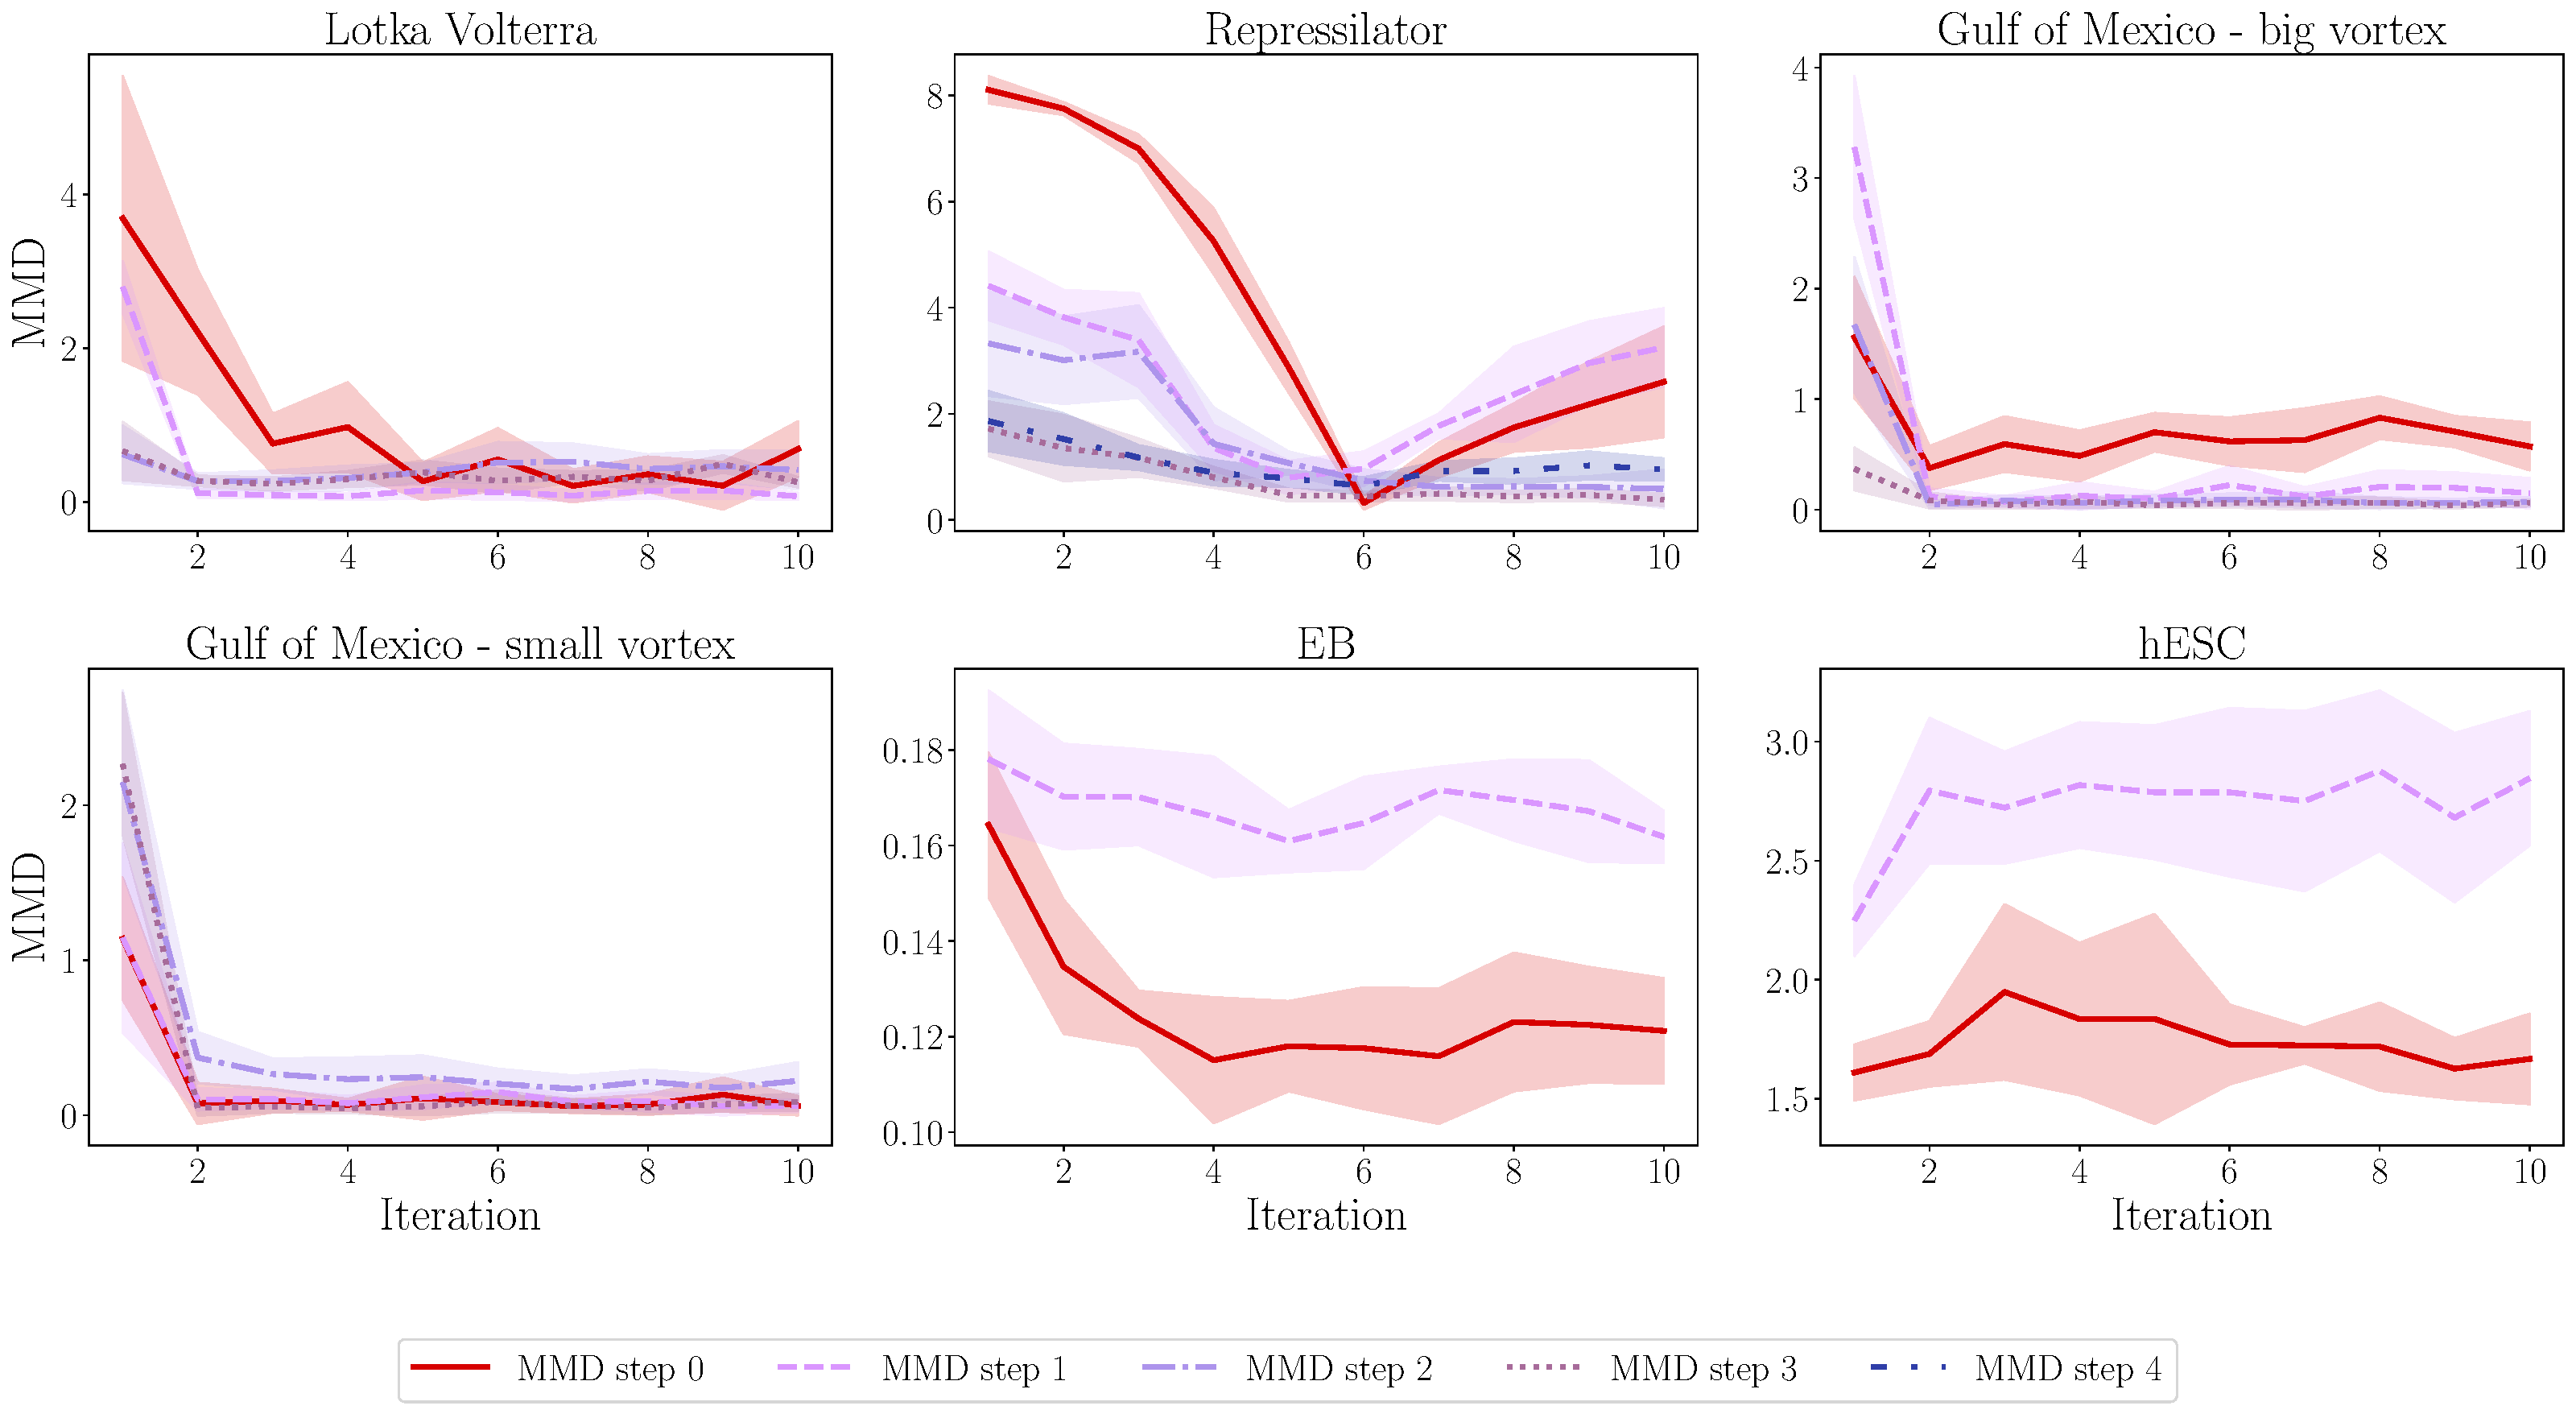
\includegraphics[width=\linewidth]{Ch3-SBIRR/Figs/MMD_eachiter_all.pdf}
    \caption{Evolution of the MMD metric across ten iterative refinement steps in our proposed method for different experimental settings. Each subplot corresponds to a specific experiment: Lotka-Volterra, Repressilator, Gulf of Mexico (big vortex), Gulf of Mexico (small vortex), EB, and hESC. The x-axis represents the iteration number, ranging from 1 to 10, while the y-axis indicates the EMD value at each validation time point. The different curves within each subplot correspond to the EMD measured at multiple validation steps.}
    \label{fig:mmditer}
\end{figure}

\clearpage

\section{Different Baselines Timing}
\label{app:timing-table}

In this section we provide a table reporting the computing times of the four methods when tested on the 6 tasks of interest. The experiments were run on four cores of Intel Xeon Gold 6248 CPU and one Nvidia Volta V100 GPU with 32 GB RAM.  

In \cref{tab:timing-tables-raw} we report the raw times for all the methods over the various tasks. The times are reported in \textbf{hours}. The format is mean $\pm$ standard deviation, where these quantities are obtained by evaluating computing times over 10 runs with 10 different seeds. We observe that \vanilla{} is the fastest method, with all tasks finishing in less than 30 minutes, and as little as few minutes for Lotka Volterra, EB, and hESC. Our method is also efficient. In general, it takes approximately 10 times longer than \vanilla{}, and this is because (1) we have to solve an SB problem $K=10$ times, and (2) the \texttt{MLEFit} step is much faster than the SB estimation itself. \dmsbname{} and TrajectoryNet are much slower. \dmsbname{} takes an average of 15 hours across all experiments, with only Lotka Volterra being a bit better (but still approximately 8 hours). TrajectoryNet takes a total of 7 to 11 hours across the various tasks. This is much slower when compared to our own method. 

To further analyze how faster our method is, we provide in \cref{tab:timing-tables-ratios} the ratios between alternative algorithms and our method's elapsed times over the different tasks. Also for this table, we provide average and standard deviation across 10 seeds. We can immediately notice that \vanilla{} is 10 times faster, as expected. \dmsbname{} ranges from being 3 to 41 times slower, with an overall average of 16 times slower across all tasks (see \cref{tab:timing-avg-avg}). TrajectoryNet performs better than \dmsbname{} but remains slower than our method, with ratios ranging from approximately 2 to 27 times slower, averaging 11 times slower overall. These results show that our method not only achieves better trajectory inference results in most experiments, but it is also much faster than all the alternatives that nontrivially handle multiple time points. We include task-specific runtime discussions in the ``Runtime" paragraphs for each experiment in \cref{ch3sec:experiments-main}.

\begin{table}[!ht]
    \centering
\begin{tabular}{|l|l|r|r|}
\toprule
algorithm & task &  mean & std \\
\midrule
\multirow[t]{9}{*}{\dmsbname} & Lotka Volterra & 7.62 & 3.18 \\
 & Repressilator & 15.63 & 0.12 \\
 & Gulf of Mexico - big vortex & 15.54 & 0.23 \\
 & Gulf of Mexico - small vortex & 15.44 & 0.02 \\
 & EB & 15.54 & 0.41 \\
 & hESC & 15.40 & 0.08 \\
 
\cline{1-4}
\multirow[t]{9}{*}{\vanilla{}} & Lotka Volterra & 0.06 & 0.01 \\
 & Repressilator & 0.23 & 0.05 \\
 & Gulf of Mexico - big vortex & 0.44 & 0.05 \\
 & Gulf of Mexico - small vortex & 0.43 & 0.01 \\
 & EB & 0.03 & $<$0.01 \\
 & hESC & 0.05 & $<$0.01 \\
 
\cline{1-4}
\multirow[t]{9}{*}{TrajectoryNet} & Lotka Volterra & 10.96 & 0.81 \\
 & Repressilator & 9.86 & 0.43 \\
 & Gulf of Mexico - big vortex & 8.10 & 0.28 \\
 & Gulf of Mexico - small vortex & 7.44 & 0.25 \\
 & EB & 10.19 & 0.37 \\
 & hESC & 8.00 & 0.49 \\
 
\cline{1-4}
\multirow[t]{9}{*}{Ours} & Lotka Volterra & 0.61 & 0.12 \\
 & Repressilator & 2.43 & 0.60 \\
 & Gulf of Mexico - big vortex & 4.68 & 0.75 \\
 & Gulf of Mexico - small vortex & 4.67 & 0.66 \\
 & EB & 0.38 & 0.05 \\
 & hESC & 0.56 & 0.04 \\
 
\bottomrule
\end{tabular}

\caption{Tables with raw timing in \textbf{hours} aggregated over 10 seeds.}
    \label{tab:timing-tables-raw}
\end{table}


\begin{table}[!ht]
    \centering
\begin{tabular}{|l|l|r|r|}
\toprule
algorithm & task &  mean & std \\
\midrule
\multirow[t]{9}{*}{\dmsbname} & Lotka Volterra & 11.98 & 6.28 \\
 & Repressilator & 6.71 & 1.25 \\
 & Gulf of Mexico - big vortex & 3.39 & 0.45 \\
 & Gulf of Mexico - small vortex & 3.36 & 0.39 \\
 & EB & 41.17 & 4.80 \\
 & hESC & 27.43 & 1.96 \\
 
\cline{1-4}
\multirow[t]{9}{*}{\vanilla{}} & Lotka Volterra & 0.10 & 0.01 \\
 & Repressilator & 0.10 & 0.01 \\
 & Gulf of Mexico - big vortex & 0.10 & 0.01 \\
 & Gulf of Mexico - small vortex & 0.09 & 0.01 \\
 & EB & 0.09 & 0.01 \\
 & hESC & 0.09 & 0.01 \\
 
\cline{1-4}
\multirow[t]{9}{*}{TrajectoryNet} & Lotka Volterra & 18.37 & 3.29 \\
 & Repressilator & 4.25 & 0.87 \\
 & Gulf of Mexico - big vortex & 1.77 & 0.25 \\
 & Gulf of Mexico - small vortex & 1.62 & 0.21 \\
 & EB & 26.97 & 2.82 \\
 & hESC & 14.26 & 1.28 \\
 
\cline{1-4}
\bottomrule
\end{tabular}

\caption{Table with the fold of acceleration of our method against alternatives (rounded to two decimal places). To compute each entry we first evaluate, for each (seed, algorithm, task) tuple, the ratio between the elapsed time for that experiment and the elapsed time for the same task and seed when our model is run. We then average these ratios across the 10 seeds and report mean and standard deviation.}
    \label{tab:timing-tables-ratios}
\end{table}



\begin{table}[!ht]
    \centering
    \begin{tabular}{|l|r|r|}
\toprule
algorithm &  mean &  std \\
\hline
                \dmsbname &        16.08 &       15.13 \\
               \vanilla{} &       0.09 &       0.01 \\
             TrajectoryNet &        11.21 &       9.72 \\
\hline
\bottomrule
\end{tabular}
    \caption{In this table, we report --- for each alternative algorithm --- average ratio speedups across all seeds and tasks. To compute this, we compute the ratios as explained in the caption of \cref{tab:timing-tables-ratios}, and then for each alternative algorithm we average these ratios over the 10 seeds and 6 tasks.}
    \label{tab:timing-avg-avg}
\end{table}

\clearpage

\section{Computational Limitations for \dmsbname\ and TrajectoryNet}
\label{app:comp-challenges}

TrajectoryNet uses continuous normalizing flows (CNFs) to model continuous-time dynamics. While CNFs are powerful for modeling complex distributions, they are often computationally intensive. Several studies have highlighted the computational challenges associated with CNFs. For example, \citet{grathwohl2018ffjord} discuss the overhead of integrating neural networks in CNFs and propose methods like FFJORD to improve efficiency. One of the key issues is that to train these methods the algorithms need to compute the trace of the Jacobian of the transformation function at each iteration. This operation is computationally expensive, especially in high-dimensional spaces \citep{chen2018neural}. The computational burden increases when regularization terms are added, as in TrajectoryNet, to enforce desired properties on the flow, further slowing down the training process.

\dmsbname{} goes beyond standard SB frameworks by tailoring the Bregman
Iteration and extending the Iteration Proportional Fitting algorithm to phase space. 
Rather than modeling particles' locations directly, this approach augments the observations with random velocities, modeling particles’ velocity and location jointly through a Langevin dynamic. We hypothesize that \dmsbname{} faces computational challenges due to learning dynamics in this expanded space (velocity and location versus location alone), as it deals with (1) the absence of direct observations for the velocity component and (2) potential inconsistencies between randomly sampled initial velocities and observed location changes (i.e., the predicted new locations using the sampled velocities may not align with the observed locations). In the context of generative modeling using diffusion, \citet{dockhorn2021score} also augment their model with particle velocities and face increased training time. 


\section{Identifiability concerns}
\label{sec:identifiability}

In some scenarios, observing marginal samples may not provide enough information to fully understand the underlying system. One situation where this can occur is when the system starts in equilibrium, such as when the initial distribution is the system's invariant measure (if one exists). However, this lack of information can also arise even when the system is not in equilibrium or when no invariant measure is present. For example, consider a system where the drift consists of a rotationally symmetric gradient field combined with a constant-curl rotational component. If the initial sample distribution is also rotationally symmetric, the marginal distribution would retain this symmetry at every time step, regardless of the angular velocity introduced by the constant-curl rotation. As a result, by only observing marginal samples, we might miss the rotational component that governs the angular velocity, preventing us from accurately inferring the system's trajectories.

\paragraph{A specific example of a rotationally invariant vector field.} Consider a vector field with constant curl, starting from an isotropic Gaussian distribution. Formally, in the context of \cref{eq:mainsde}, consider a simple two-dimensional drift $\drift(\bm{x}) = [\alpha x_2, -\alpha x_1]^\top$,
where \(\alpha \in \mathbb{R}\) is a parameter. This represents the dynamics of a vector field with constant curl. When \(\alpha = 0\), the system is purely driven by Brownian motion. Then assume the initial distribution \(\marginal{0}\) is isotropic normal, i.e., \(\marginal{0} \sim \mathcal{N}(0, \beta I_2)\) for some \(\beta\), where \(I_2\) is the 2D identity matrix. For a fixed volatility \(\gamma\), when \(\alpha = 0\), the particle distribution at any future time step remains an isotropic normal distribution.

Indeed, if we consider the general form of the Fokker--Planck equation,
\begin{align*}
    \frac{\partial p(\bm x, t)}{\partial t}
    = -\nabla\cdot \bigl(\drift(\bm x)\,p(\bm x, t)\bigr)
      + \gamma \nabla^2 p(\bm x, t)
    = - p(\bm x, t) \,\bigl(\nabla\cdot \drift(\bm x)\bigr)
      - \nabla p(\bm x, t)\cdot \drift(\bm x)
      + \gamma \nabla^2 p(\bm x, t),
\end{align*}
we see that for this isotropic Gaussian setting, \(\nabla p(\bm x, t)\cdot \drift(\bm x)=0\). Hence only the diffusion term remains, and the distribution of the particles at any time step stays isotropic Gaussian with increasing variance. Schrödinger bridges between these Gaussians have a unique closed-form \citep{Bunne2023}, which cannot account for all possible rotations. This illustrates how certain symmetries (like rotational invariance) can lead to multiple vector fields that produce indistinguishable marginal or trajectory behaviors under certain conditions.

\paragraph{Two Types of Identifiability Concerns.} The above example underscores the broader issue that different underlying systems can give rise to the same observed data. We identify at least two distinct scenarios:

\begin{itemize}
    \item \textbf{(1) Different systems yielding the \emph{same} trajectory.} Two (or more) truly distinct underlying dynamics might coincide on the \emph{exact} same trajectory over time. In this situation, identifying which system actually generated the data is strictly harder (and in some cases, impossible) given only trajectory observations. However, note that \emph{identifying} the system is a different goal from simply producing accurate predictions or interpolations. It is possible to infer a usable trajectory even when the true system remains ambiguous.
    \item \textbf{(2) Different dynamics yielding the same marginal distributions at observed time points, but differing in-between.}
    Even if one has marginals at a few discrete time points, different dynamics can ``fill in'' between these marginals in different ways, leading to distinct trajectories that match the same observed endpoints. This poses a fundamental limitation for trajectory inference unless additional information (e.g., domain knowledge or more finely sampled data) is introduced. Providing uncertainty quantification over all plausible trajectories could be an interesting way to reflect this ambiguity.
\end{itemize}

These concerns mirror those in inverse problems and PDE identifiability. For instance, \citet{lavenant2024toward} showed that if one has marginals sampled arbitrarily densely in time (and the vector field is a gradient field), then the trajectories can indeed be uniquely identified. \citet{guan2024identifying} provide conditions under which a system with \emph{linear drift} and \emph{additive diffusion} can be identified from snapshot data, specifically when the initial distribution is not invariant to a class of generalized rotations. These results demonstrate that identifiability can hold under certain conditions but also indicate how quickly it may fail under symmetries or insufficient sampling.

\paragraph{Relation to Convergence in \Cref{prop:iter-kl}}

In \cref{prop:iter-kl}, we show that the KL divergence in our iterative method is guaranteed to converge because the sequence it forms is a lower-bounded, monotonically decreasing sequence. However, this does not imply that the \emph{arguments} of the KL (i.e., the pair \((p,q)\)) necessarily converge to a \emph{unique} solution. In principle, there could be multiple \((p,q)\) pairs that produce the same KL value and are equally consistent with the observed data. In other words, this is precisely an \emph{identifiability issue}: if multiple solutions fit the same marginal distributions (and/or constraints) equally well, the algorithm might either settle on different solutions depending on initialization or potentially ``cycle'' among equivalent solutions. While we
do not observe such cycling in our experiments, it remains an open theoretical question whether this cycling could occur. Ensuring uniqueness of the solution beyond the decreasing KL criterion may demand additional constraints, richer data sampling, or stronger prior assumptions. We believe investigating these settings, and the broader issue of identifiability, is a fruitful direction for future research.

